\documentclass[12pt]{article}

\usepackage[letterpaper, margin=0.75in, includeheadfoot, centering,
headsep=1.5ex, headheight=15pt]{geometry}

\linespread{1.0}
\setlength{\parskip}{0.5ex}
%\setlength{\parindent}{0in}

\usepackage[protrusion=true,expansion=true]{microtype}
\usepackage[T1]{fontenc}
\usepackage[bitstream-charter]{mathdesign} % Charter BT

\usepackage[compact]{titlesec}
\titlespacing*{\section}{0pt}{*0}{*0}
\titleformat*{\section}{\large\bfseries}
\titlespacing*{\subsection}{0pt}{*0}{*0}
\titlespacing*{\subsubsection}{0pt}{*0}{*0}

\usepackage{fancyhdr}
\pagestyle{fancy}
\fancyhead{}
\fancyfoot{}
\chead{}
\lhead{Grant Title Goes Here}
\rhead{John. H. Smith}
\cfoot{\thepage}

\usepackage{graphicx}
\usepackage[labelfont=bf, skip=3ex, width=0.9\textwidth]{caption}

\usepackage{citecollapse}
\let\oldthebibliography=\thebibliography
\let\endoldthebibliography=\endthebibliography
\renewenvironment{thebibliography}[1]{%
  \begin{oldthebibliography}{#1}%
    \setlength{\parskip}{0ex}%
    \setlength{\itemsep}{0.75ex}%
}%
{%
  \end{oldthebibliography}%
}

\usepackage{lipsum}

\begin{document}
  
\section*{Introduction}

As in \cite{mattar2005motor} and in \cite{hodgkin1952propagation},
and as seen in Figure~\ref{fig:robot}, \lipsum[1-5]

\section*{General Methods}

\lipsum[1-5]

\newpage
\bibliography{refs}
\bibliographystyle{ieeetr}


\newpage
\clearpage
\begin{figure}[H]
	\centering
        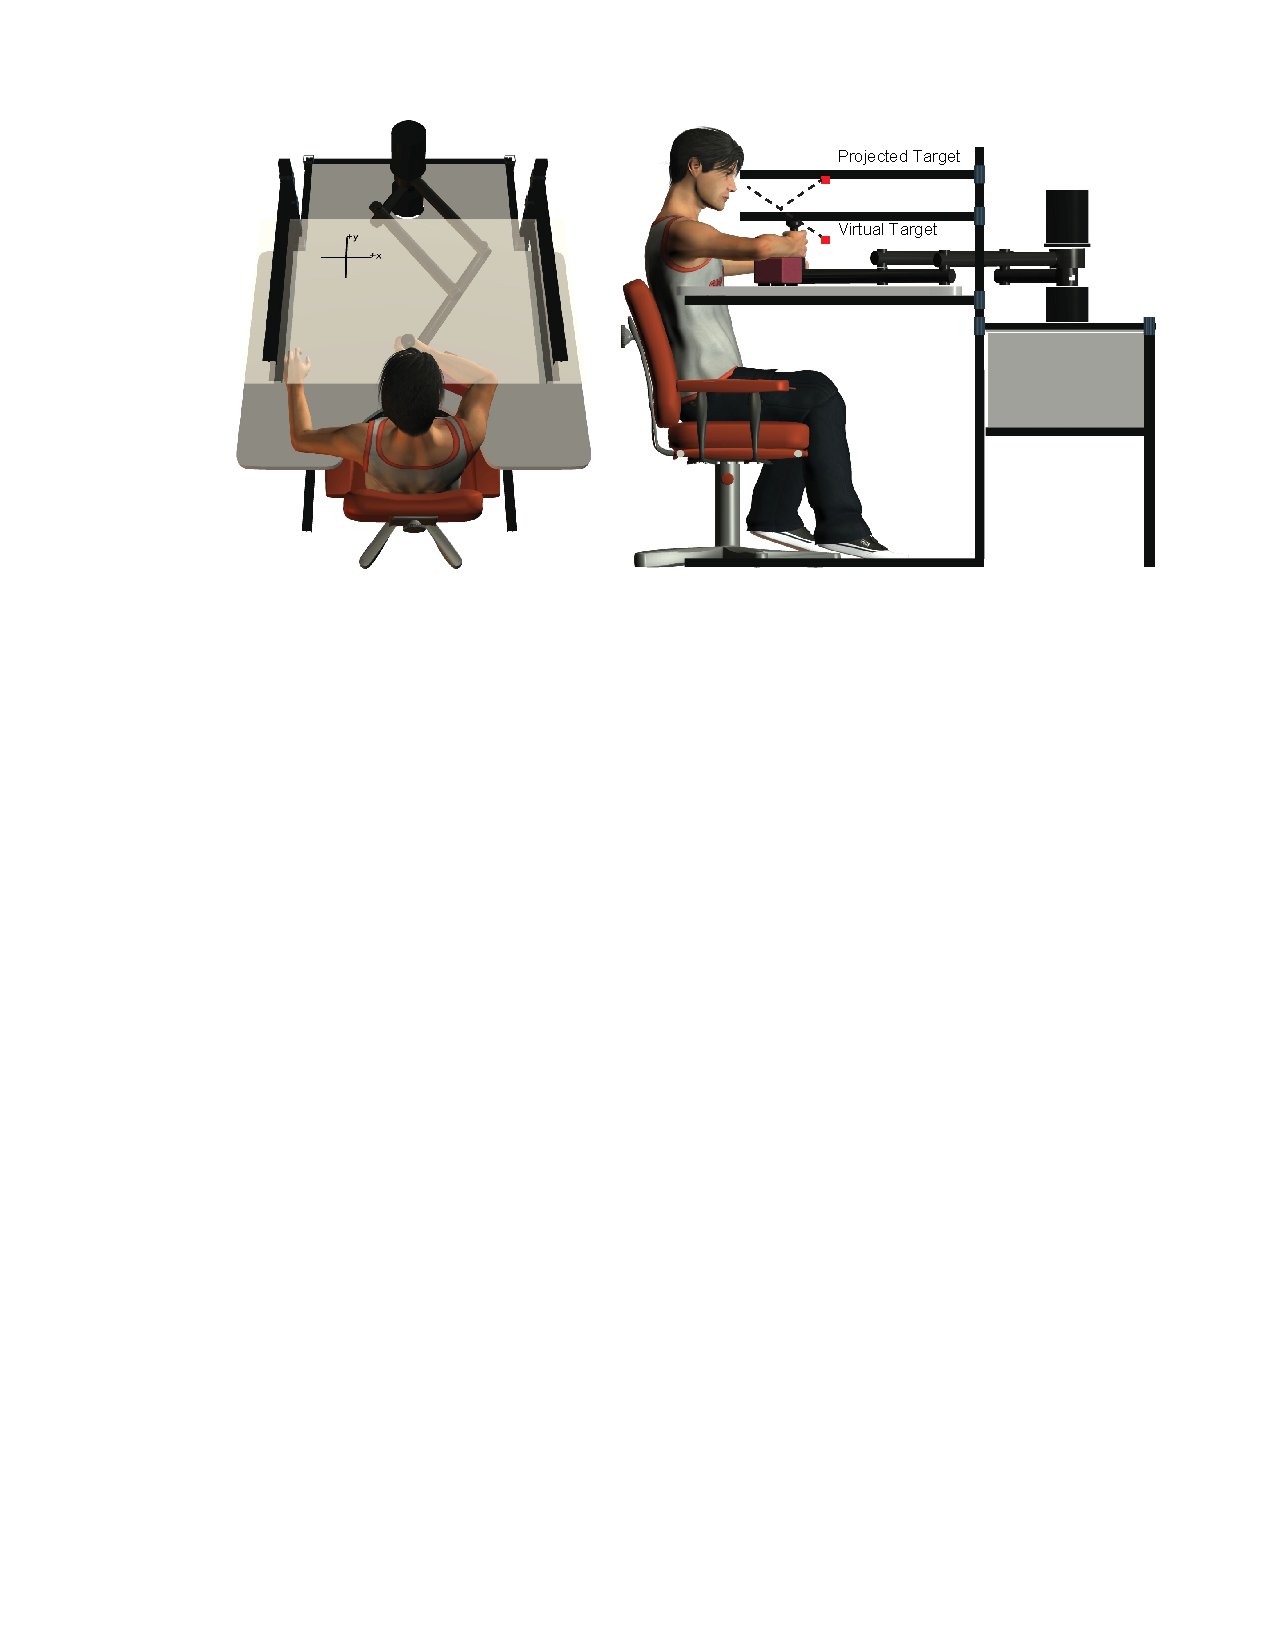
\includegraphics[height=3in]{robot_imt.pdf}
        \caption{\textbf{Endpoint Robot}. The IMT2 endpoint robot
          allows for arm movement (shoulder and elbow rotation) in a
          horizontal plane. Positions are measured using optical
          encoders, and forces applied by the subject at the robot
          handle are measured using a 6D ATI force/torque
          transducer. Signals are digitized at 500Hz. Time-varying
          forces applied by the robot may be specified as a function
          of limb position, velocity, acceleration and force. Muscle
          activation patterns are detected using surface
          electromyographic (EMG) electrodes (Delsys Inc., Boston) and
          digitized at 1000Hz.}
 \label{fig:robot}
\end{figure}


%\newpage
%\clearpage
%\begin{figure}[H]
%	\centering
%        \includegraphics[height=4in]{}
%        \caption{\textbf{Caption Title}. Caption goes here.}
% \label{}
%\end{figure}


\end{document}
